\begin{figure}
    \centering
    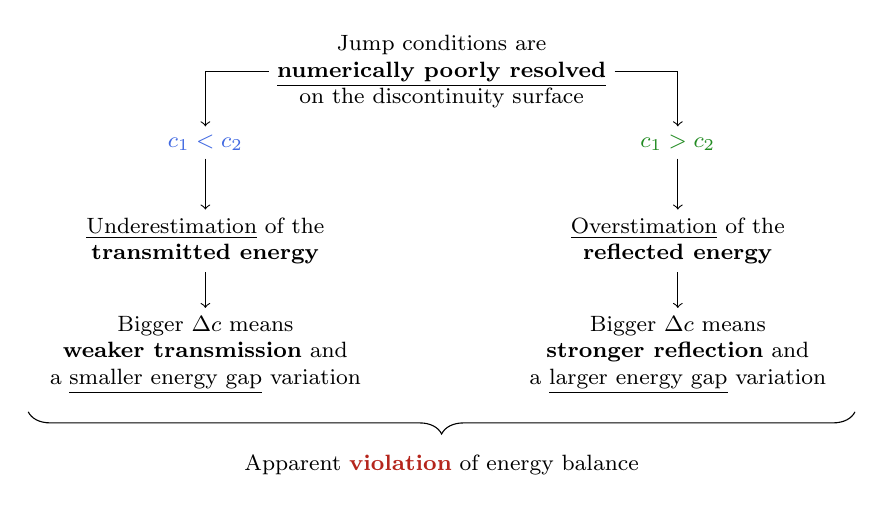
\begin{tikzpicture}
        \footnotesize

        \node[align=center] at (0,5) (A) {Jump conditions are\\ \textbf{\underline{numerically poorly resolved}}\\ on the discontinuity surface};

        \node at (-3,4.1) (B) {$\textcolor{RoyalBlue}{\boldsymbol{c_1<c_2}}$};
        \node at (3,4.1) (C) {$\textcolor{ForestGreen}{\boldsymbol{c_1>c_2}}$};

        \node[align=center] at (-3,2.85) (D) {\underline{Underestimation} of the\\ \textbf{transmitted energy}};
        \node[align=center] at (3,2.85) (E) {\underline{Overstimation} of the\\ \textbf{reflected energy}};

        \node[align=center] at (-3,1.4) (F) {Bigger $\Delta c$ means\\ \textbf{weaker transmission} and \\ a \underline{smaller energy gap} variation};
        \node[align=center] at (3,1.4) (G) {Bigger $\Delta c$ means\\ \textbf{stronger reflection} and\\ a \underline{larger energy gap} variation};

        \draw[->] (A) -- (-3,5) -- (B);
        \draw[->] (A) -- (3,5) -- (C);
        \draw[->] (B) -- (D);
        \draw[->] (C) -- (E);
        \draw[->] (D) -- (F);
        \draw[->] (E) -- (G);

        \draw[decorate, decoration={brace, amplitude=8pt, raise=2pt}] (5.25,0.75) -- (-5.25,0.75);

        \node at (0,0) () {Apparent \textcolor{BrickRed}{\textbf{violation}} of energy balance};

        \normalsize
    \end{tikzpicture}
\end{figure}